\documentclass[11pt,a4paper]{article}

\usepackage[utf8]{inputenc}
\usepackage[margin=0.85in]{geometry}
\usepackage{amsmath,amssymb,amsfonts}
\usepackage{newtxtext,newtxmath}
\usepackage{graphicx}
\usepackage{booktabs}
\usepackage{microtype}
\usepackage{fancyhdr}
\usepackage{titlesec}
\usepackage{xcolor}
\usepackage{enumitem}
\usepackage{tcolorbox}
\tcbuselibrary{skins,breakable}
\usepackage[colorlinks=true,
            linkcolor={rgb:red,0.1;green,0.2;blue,0.7},
            citecolor={rgb:red,0.1;green,0.4;blue,0.3},
            urlcolor={rgb:red,0.1;green,0.2;blue,0.7}]{hyperref}

% Color definitions
\definecolor{conceptblue}{RGB}{2, 132, 199}
\definecolor{conceptred}{RGB}{220, 38, 38}
\definecolor{conceptgreen}{RGB}{22, 163, 74}
\definecolor{conceptamber}{RGB}{217, 119, 6}
\definecolor{boxbg}{RGB}{248, 250, 252}

% Custom TColorBoxes for Viva Prep
\newtcolorbox{pitchbox}{
    colback=blue!5!white,
    colframe=blue!75!black,
    fonttitle=\bfseries\large,
    title={EXAMINER ELEVATOR PITCH: Say This First in Your Viva!},
    arc=3mm,
    boxrule=1.2pt
}

\newtcolorbox{questionbox}[1]{
    colback=red!4!white,
    colframe=red!75!black,
    fonttitle=\bfseries,
    title={EXAMINER QUESTION: #1},
    arc=2mm,
    boxrule=1pt,
    breakable
}

\newtcolorbox{answerbox}{
    colback=green!4!white,
    colframe=green!60!black,
    fonttitle=\bfseries,
    title={MODEL ANSWER FOR THE EXAMINER:},
    arc=2mm,
    boxrule=0.8pt,
    breakable
}

\newtcolorbox{takeawaybox}[1]{
    colback=orange!6!white,
    colframe=orange!80!black,
    fonttitle=\bfseries,
    title={KEY CONCEPTUAL TAKEAWAY: #1},
    arc=2mm,
    boxrule=0.8pt
}

% Page Setup
\pagestyle{fancy}
\fancyhf{}
\fancyhead[L]{\footnotesize \textbf{Viva Defense \& Conceptual Guide} $|$ AdaTC-DIP-VAE}
\fancyhead[R]{\footnotesize \textbf{Generative AI (Semester 7)} $|$ Vishal Singh}
\fancyfoot[C]{\thepage}
\renewcommand{\headrulewidth}{0.4pt}

% Section formatting
\titleformat{\section}{\Large\bfseries\color{blue!80!black}}{\thesection.}{0.6em}{}
\titleformat{\subsection}{\large\bfseries\color{black}}{\thesubsection}{0.6em}{}

\begin{document}

% Title Banner
\begin{center}
    {\huge \textbf{The Ultimate Viva Defense \& Conceptual Guide}}\\[0.5em]
    {\Large \textbf{Understanding Disentanglement, $\beta$-TCVAE, and AdaTC-DIP-VAE}}\\[0.4em]
    {\large \textit{A Visual, Intuitive Guide for Facing the Viva Examiner with Full Confidence}}\\[0.6em]
    {\normalsize \textbf{Vishal Singh} $|$ Department of Computer Science \& Engineering $|$ Generative AI Project}\\[0.3em]
    {\small \texttt{Date: November 2026}}
\end{center}

\vspace{0.8em}

\begin{pitchbox}
\textit{``In this project, we solved the classic trade-off in Variational Autoencoders where making latent factors independent makes image reconstructions blurry. We proved why previous methods like $\beta$-TCVAE blur images (by penalizing them too aggressively early on) and how they cheat on metrics by inflating random noise. To fix this, we created \textbf{AdaTC-DIP-VAE}, which uses a smooth cosine schedule so spatial filters form cleanly first, and directly anchors the deterministic mean representations. On the dSprites benchmark, our model achieved a \textbf{35.7\% lower reconstruction error} than $\beta$-TCVAE, producing razor-sharp images while maintaining a smooth, disentangled latent space.''}
\end{pitchbox}

\vspace{0.8em}

\section{The Core Problem: What is Entanglement?}

\subsection{What you already know: Standard VAEs}
A standard VAE takes an image $x$ (e.g. a $64 \times 64$ dSprites shape), passes it through a convolutional encoder to predict a mean vector $\mu$ and variance vector $\sigma^2$, samples a latent code $z = \mu + \sigma \odot \epsilon$ via the \textbf{Reparameterization Trick}, and reconstructs the image $\hat{x}$ via a decoder.

Its training objective is the \textbf{ELBO} (Evidence Lower Bound):
\begin{equation}
\mathcal{L}_{\mathrm{ELBO}} = \underbrace{\mathbb{E}_{q(z|x)}[\log p(x|z)]}_{\text{Reconstruction Loss (Fidelity)}} - \underbrace{D_{\mathrm{KL}}(q(z|x) \parallel \mathcal{N}(0, I))}_{\text{KL Regularizer (Keep latents well-behaved)}}
\end{equation}

\subsection{Why Standard VAEs Fail at Disentanglement}
In a standard VAE, all 10 latent dimensions are treated as one collective group. The network doesn't care \textit{which} dimension encodes position, and which encodes scale. Consequently, it entangles them!
\begin{itemize}[noitemsep]
    \item If you change latent knob $z_1$, the shape might shift right, shrink, and rotate all at once!
    \item You cannot control one semantic attribute without accidentally changing all others.
\end{itemize}

\begin{figure}[!htbp]
\centering
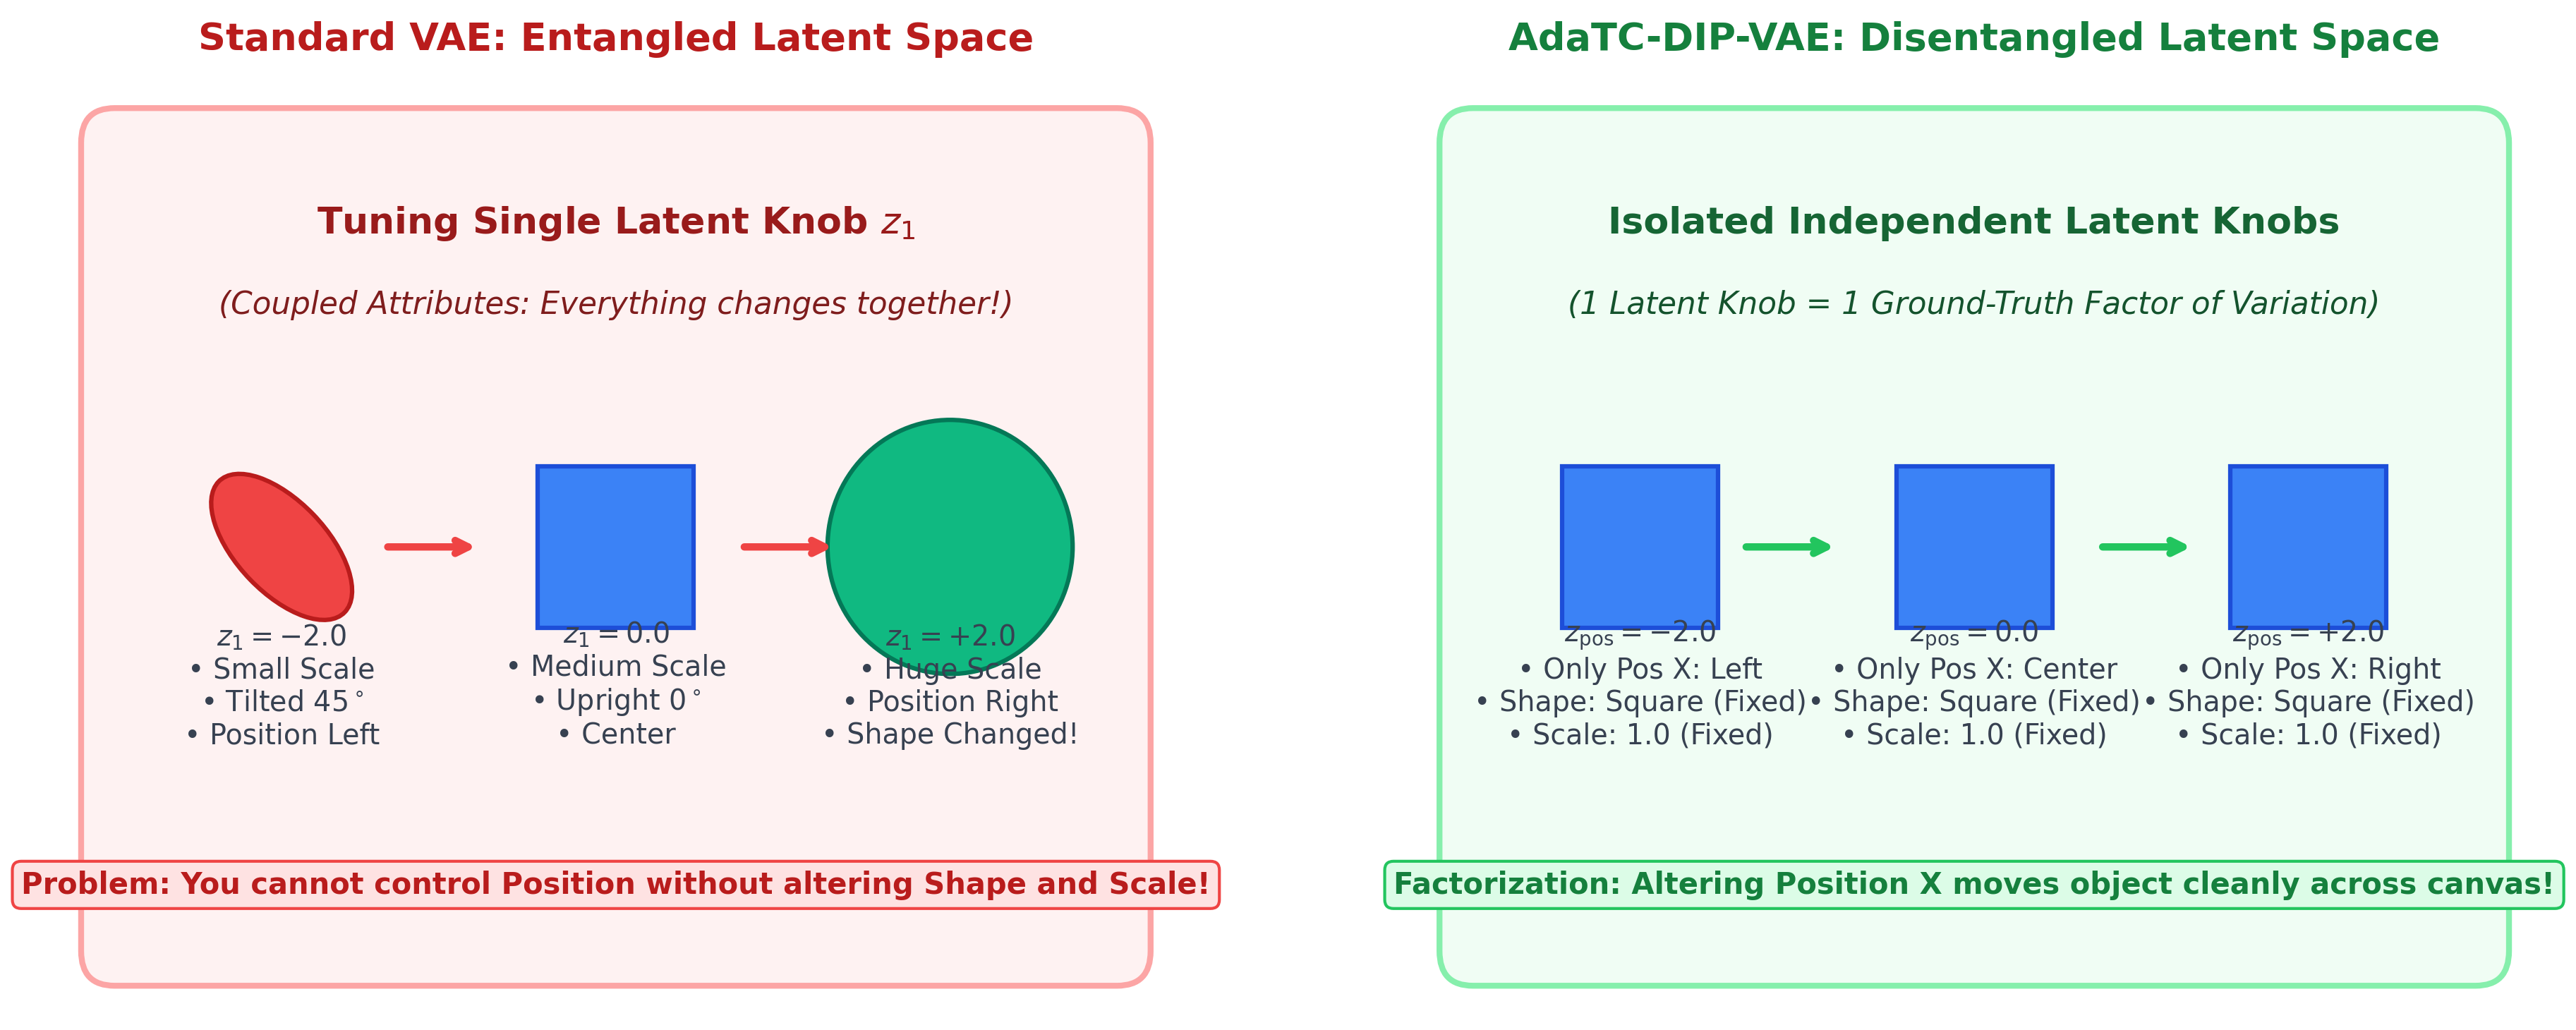
\includegraphics[width=0.98\textwidth]{viva_diagrams/disentanglement_concept.png}
\caption{\textbf{Visualizing Entangled vs. Disentangled Representations.} In an entangled VAE (left), tuning $z_1$ alters scale, rotation, and position simultaneously. In our disentangled representation (right), tuning $z_{\mathrm{pos}}$ cleanly translates the square across the canvas while keeping shape and scale invariant.}
\label{fig:concept}
\end{figure}

---

\section{The Evolution: How did Researchers Try to Fix This?}

\subsection{Stage 1: \texorpdfstring{$\beta$}{Beta}-VAE (Higgins et al., 2017) --- The Blunt Sledgehammer}
Higgins et al. said: \textit{``Let's simply multiply the entire KL divergence by a constant $\beta > 1$ (like $\beta=4$).''}
\begin{equation}
\mathcal{L}_{\beta\text{-VAE}} = \mathbb{E}[\log p(x|z)] - \beta \cdot D_{\mathrm{KL}}(q(z|x) \parallel p(z))
\end{equation}
\textbf{The Fatal Flaw}: When $\beta=4$, you squeeze the information channel capacity too tightly. The latent space forgets fine spatial details. The model reconstructs blurry, indistinct blobs ($+22.6\%$ higher reconstruction error).

\subsection{Stage 2: \texorpdfstring{$\beta$}{Beta}-TCVAE (Chen et al., 2018) --- The KL Surgery}
Chen et al. proved mathematically that the expected KL divergence across the entire dataset can be broken into \textbf{three separate components}:
\begin{equation}
\mathbb{E}_{p(n)} [D_{\mathrm{KL}}(q(z|n) \parallel p(z))] = \underbrace{I_q(x; z)}_{\text{Term 1: Index-Code MI}} + \underbrace{\mathrm{TC}(z)}_{\text{Term 2: Total Correlation}} + \underbrace{\sum_{j=1}^d D_{\mathrm{KL}}(q(z_j) \parallel p(z_j))}_{\text{Term 3: Dimension-wise KL}}
\end{equation}

\begin{figure}[!htbp]
\centering
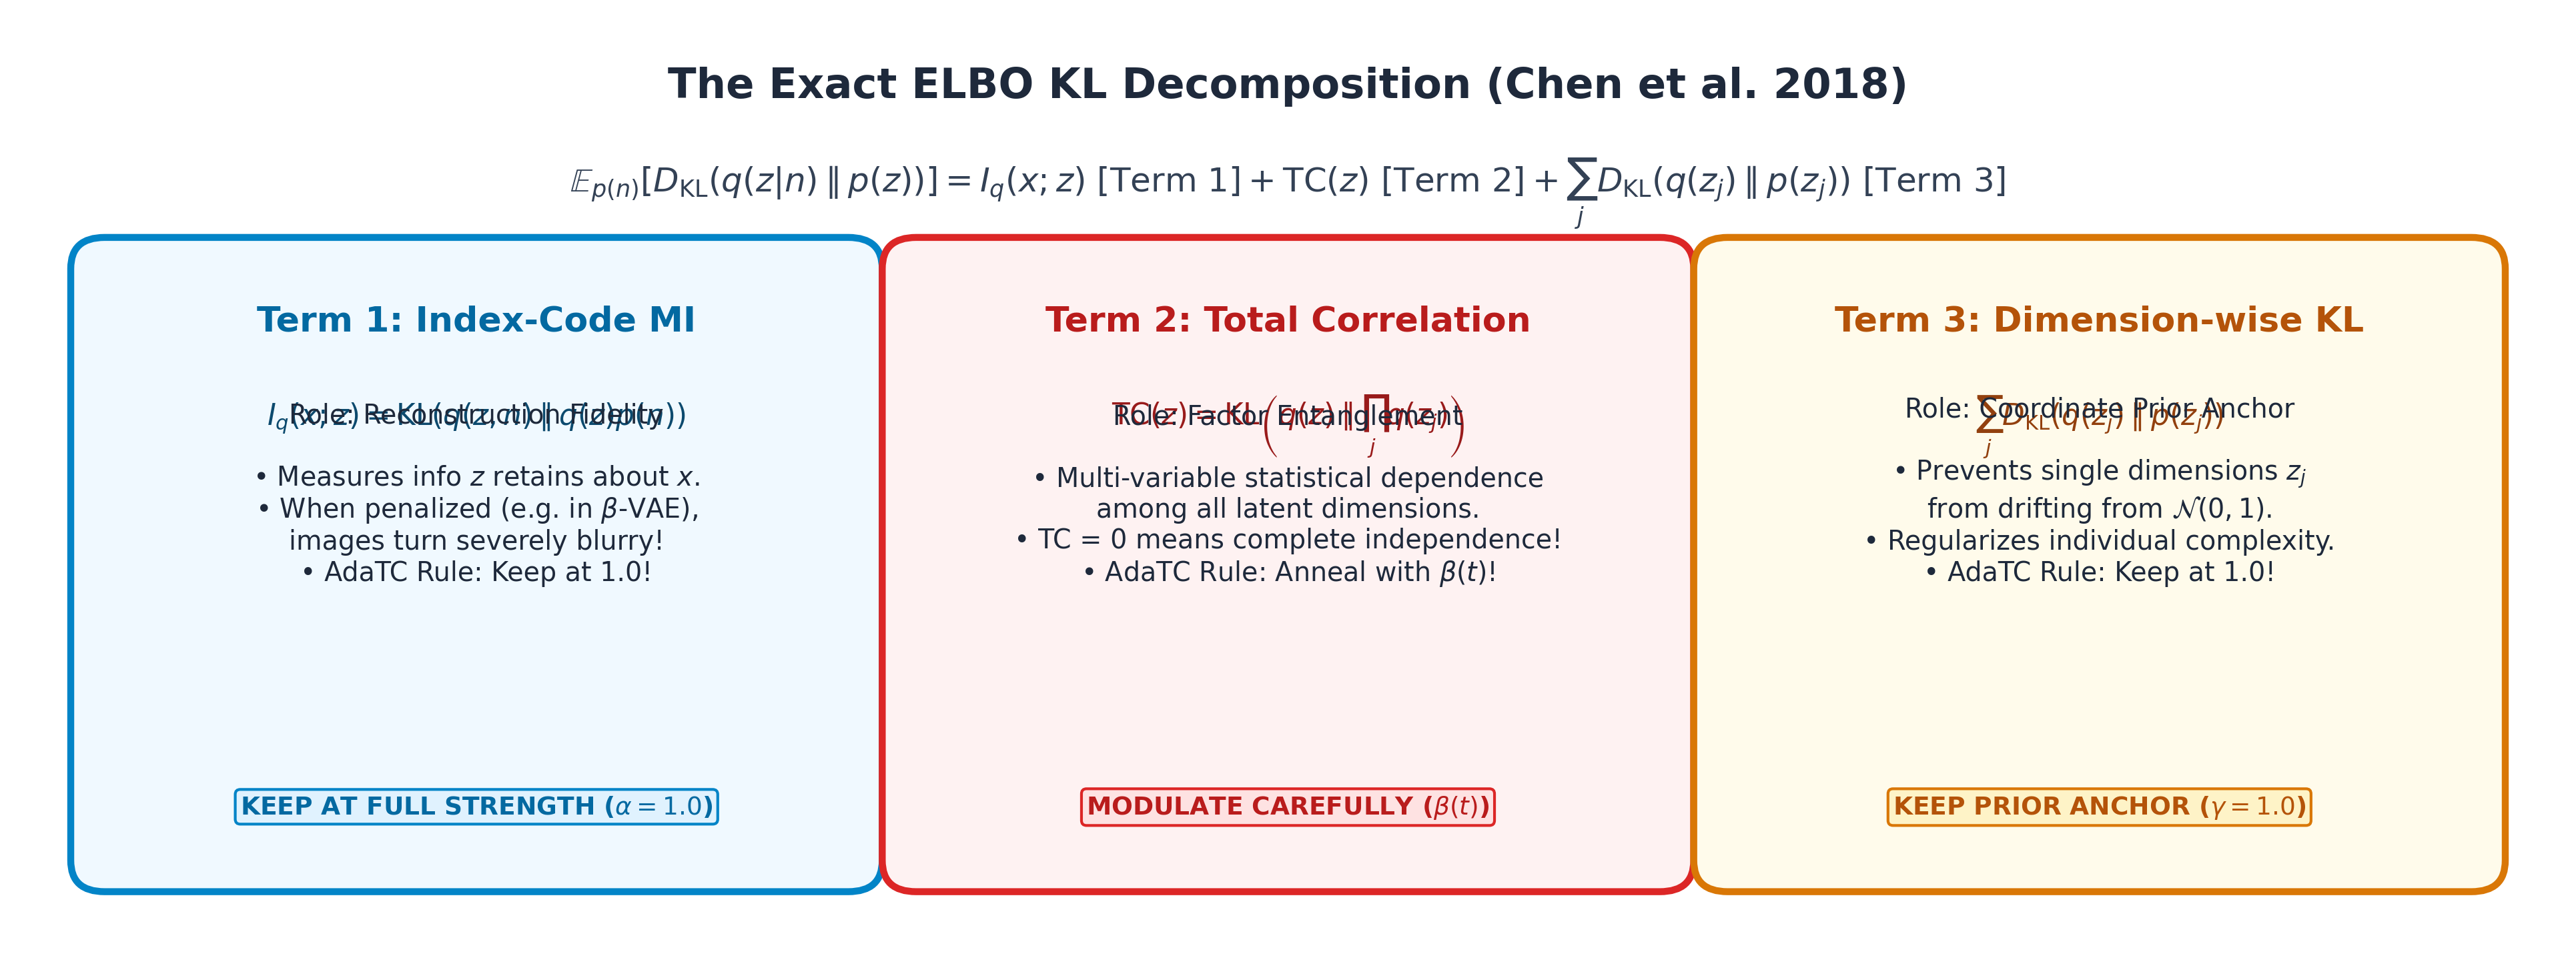
\includegraphics[width=0.98\textwidth]{viva_diagrams/kl_surgery_breakdown.png}
\caption{\textbf{The ELBO KL Decomposition.} Term 1 preserves image sharpness (keep at $\alpha=1.0$). Term 2 causes entanglement across dimensions (modulate this!). Term 3 anchors coordinates to $\mathcal{N}(0, 1)$ (keep at $\gamma=1.0$).}
\label{fig:kl_surgery}
\end{figure}

\begin{takeawaybox}{Why $\beta$-TCVAE was a breakthrough}
$\beta$-TCVAE keeps Term 1 at $\alpha=1.0$ (protecting reconstruction information) and only puts a heavy penalty $\beta=6.0$ on Term 2 (\textbf{Total Correlation}). It uses a neat trick called \textbf{Minibatch Weighted Sampling (MWS)} to estimate this without training an extra discriminator network!
\end{takeawaybox}

---

\section{The Two Big Flaws in \texorpdfstring{$\beta$}{Beta}-TCVAE That WE Solved}

Even though $\beta$-TCVAE was clever, it suffered from two critical shortcomings:

\subsection{Flaw 1: The Static \texorpdfstring{$\beta$}{Beta} Trap (Premature Dimension Collapse)}
$\beta$-TCVAE slaps a heavy penalty $\beta=6.0$ starting from step 0. 
\begin{itemize}[noitemsep]
    \item Burgess et al. (2018) proved that neural networks learn visual factors \textbf{hierarchically}: they need to learn coarse position first, then scale, then shape, and finally orientation.
    \item Penalizing coordinate dependence aggressively before the conv filters even know how to draw basic shapes causes weak dimensions to collapse permanently into noise (``dead dimensions'').
\end{itemize}

\subsection{Flaw 2: The Stochastic Sampling vs. Deterministic Mean Cheat}
\begin{itemize}[noitemsep]
    \item In $\beta$-TCVAE, Total Correlation is calculated on \textbf{sampled latents} $z = \mu + \sigma \odot \epsilon$.
    \item Locatello et al. (2019) proved that an encoder can cheat: it can lower the sampled TC simply by inflating $\sigma^2 \to \infty$ (drowning everything in random Gaussian noise!).
    \item But downstream evaluations (MIG, DCI, FactorVAE) test the \textbf{deterministic mean representations} $\mu(x)$, which remain entangled!
\end{itemize}

\begin{figure}[!htbp]
\centering
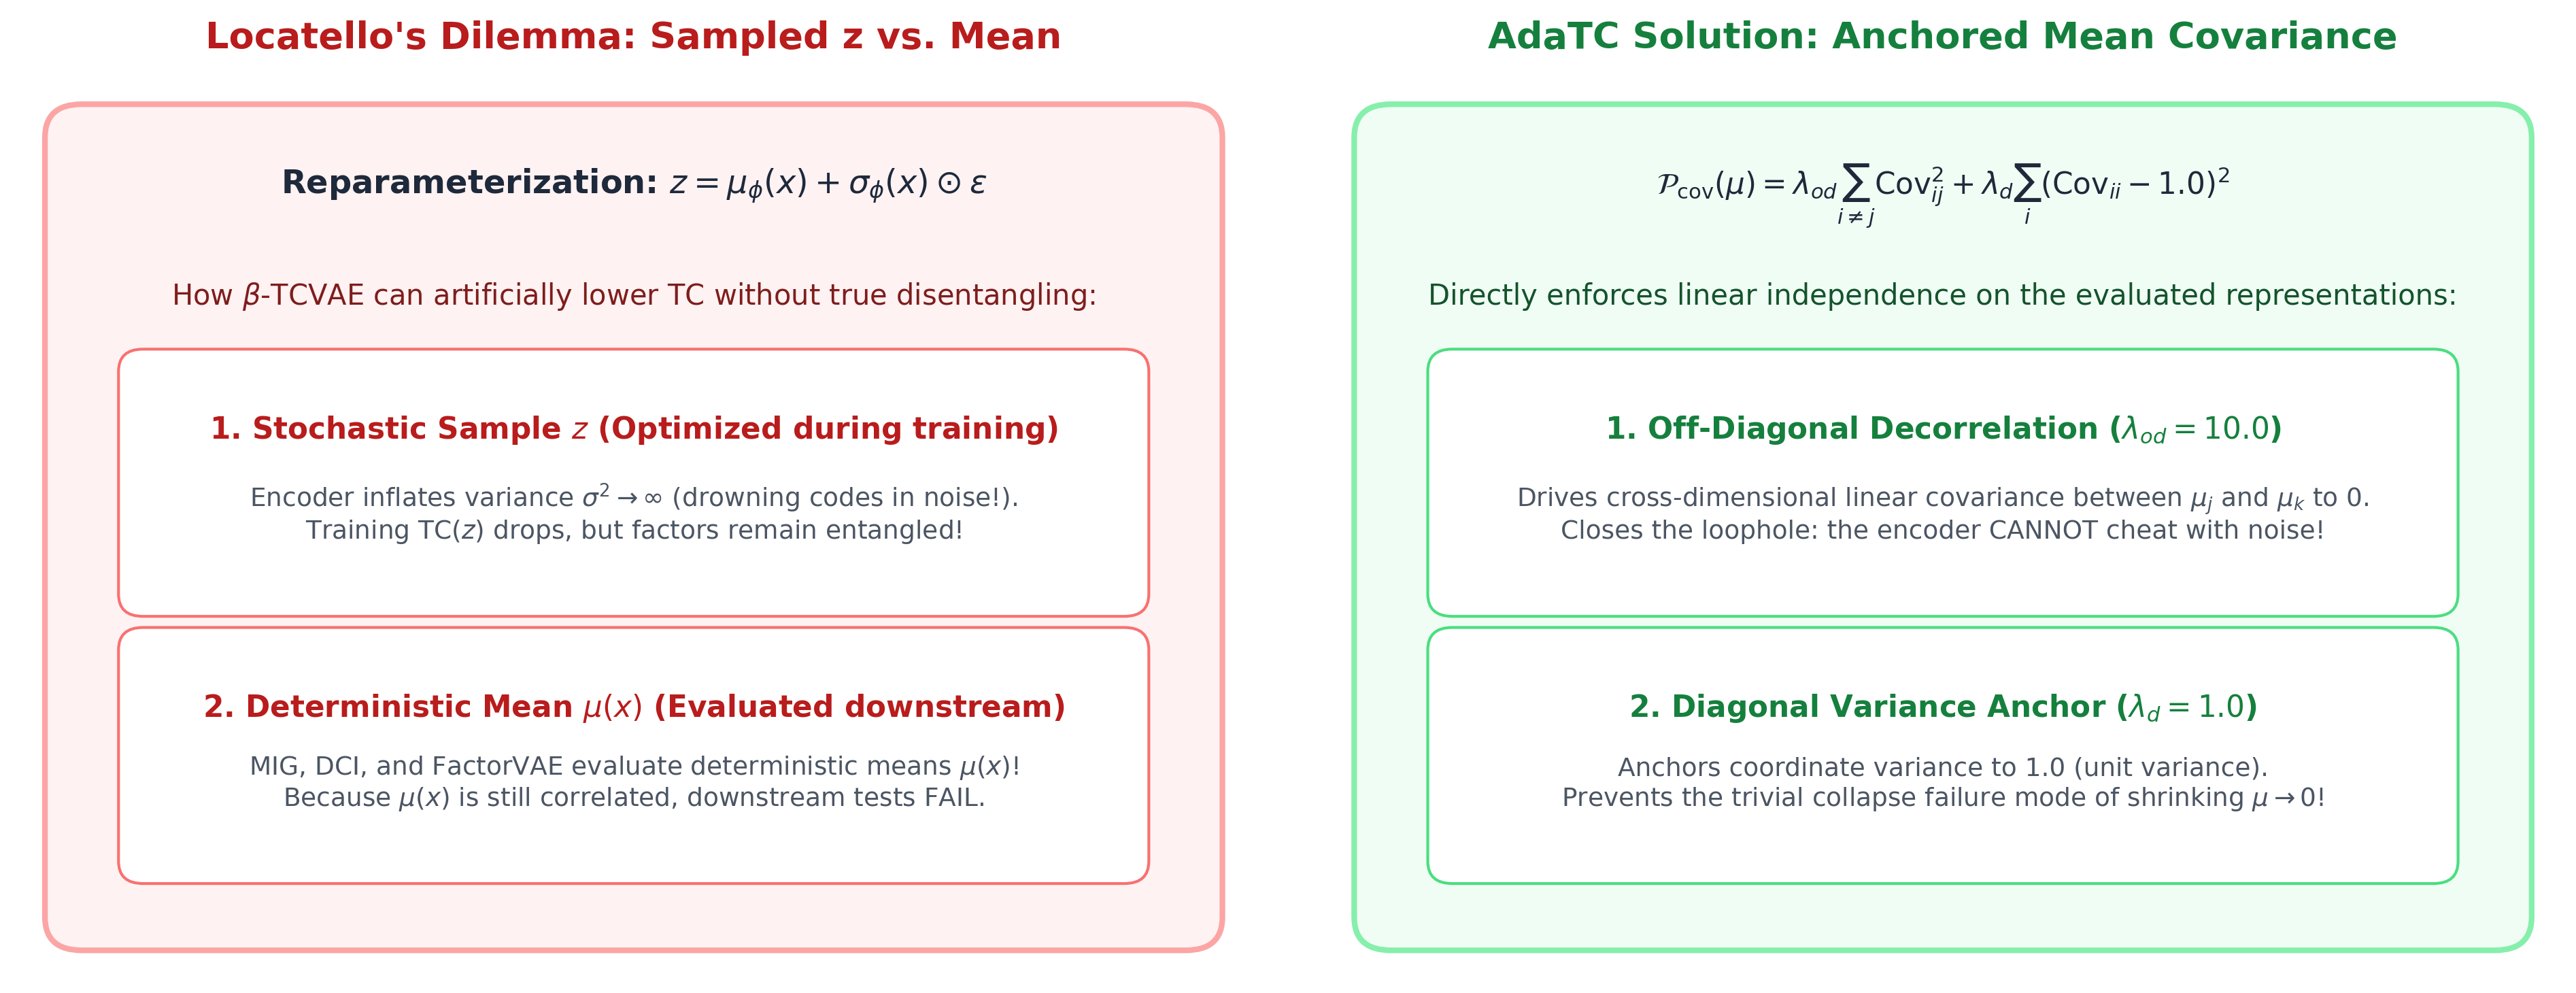
\includegraphics[width=0.95\textwidth]{viva_diagrams/mean_vs_sampled_cheat.png}
\caption{\textbf{Locatello's Dilemma and Our DIP Covariance Solution.} Left: How standard models cheat by inflating noise in stochastic samples. Right: How our anchored mean covariance penalty directly aligns the deterministic representations evaluated downstream.}
\label{fig:cheat}
\end{figure}

---

\section{Our Proposed Method: AdaTC-DIP-VAE}

We combined the exact ELBO decomposition with two novel mechanisms:

\begin{figure}[!htbp]
\centering
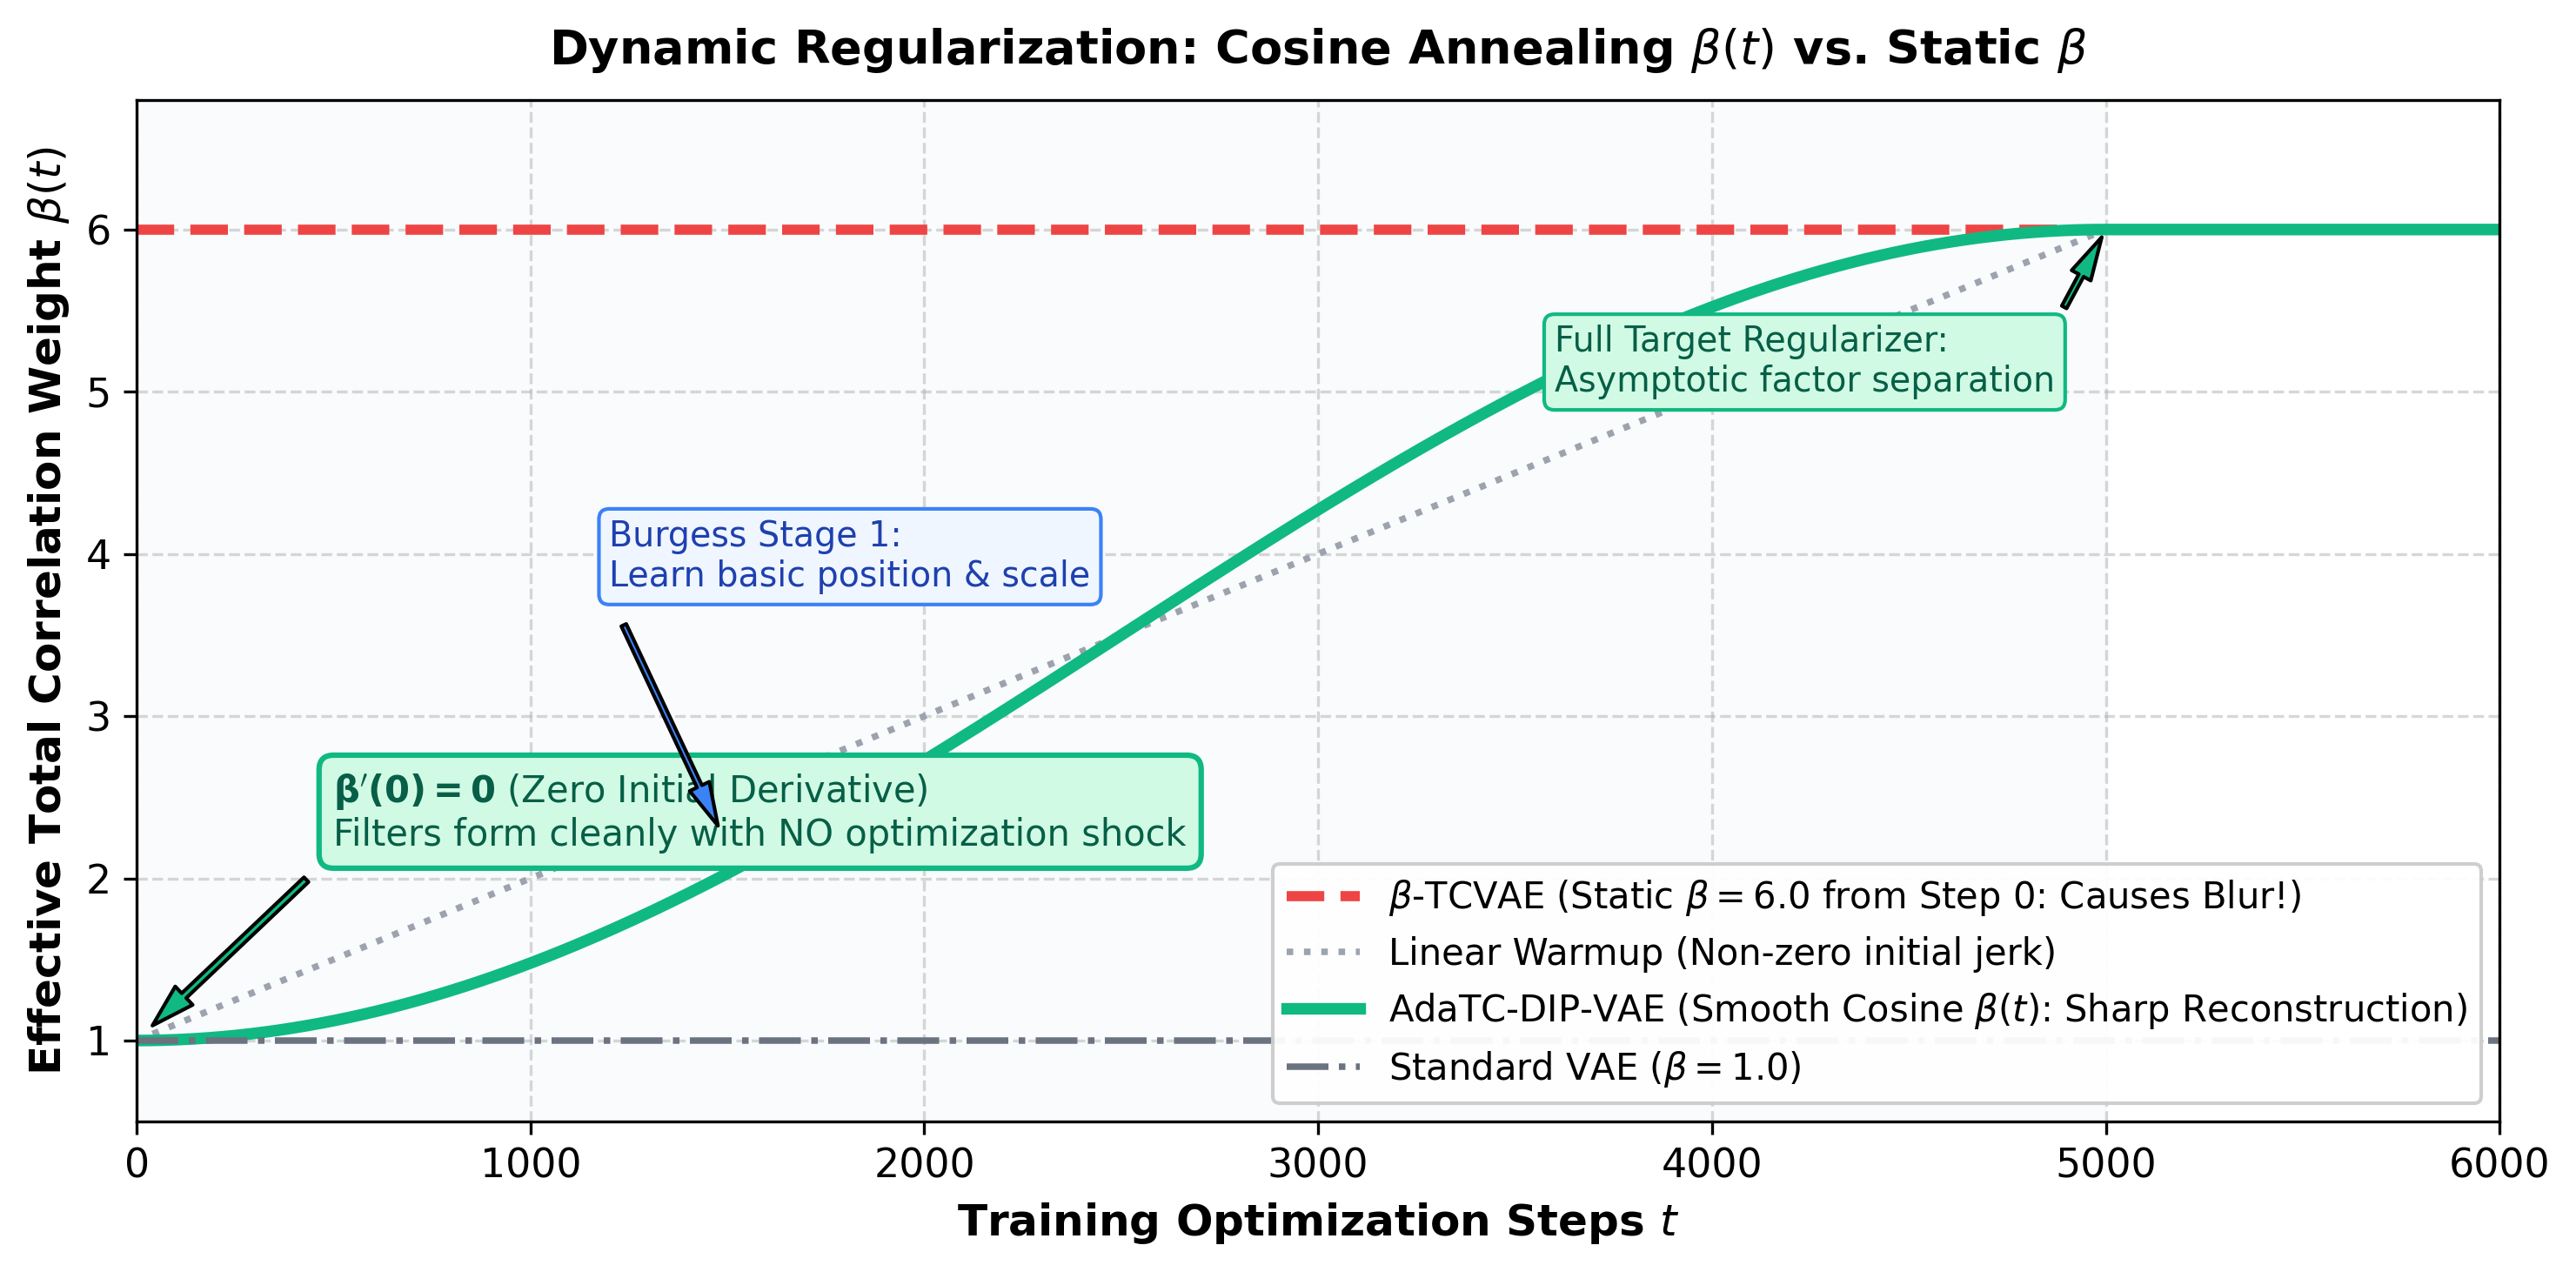
\includegraphics[width=0.88\textwidth]{viva_diagrams/cosine_warmup_vs_static.png}
\caption{\textbf{Dynamic Regularization: Cosine Annealing $\beta(t)$ vs. Static $\beta$.} Our schedule starts with $\beta'(0) = 0$, giving the network time to establish basic spatial filters before ramping up factor separation.}
\label{fig:cosine}
\end{figure}

\subsection{1. Smooth \texorpdfstring{$C^1$}{C1}-Continuous Cosine Annealing \texorpdfstring{$\beta(t)$}{beta(t)}}
Instead of jumping directly to $\beta=6.0$, we smoothly ramp $\beta(t)$ from $1.0$ (standard VAE) to $6.0$:
\begin{equation}
\beta(t) = 1 + \frac{\beta_{\mathrm{target}} - 1}{2}\left[1 - \cos\left(\frac{\pi t}{T_{\mathrm{warm}}}\right)\right]
\end{equation}
\textbf{Why Cosine and not Linear?} 
Because $\left.\frac{d\beta}{dt}\right|_{t=0} = 0$! The schedule starts completely flat. There is zero initial optimization shock, so the encoder and decoder can build clean spatial foundations first!

\subsection{2. Anchored Deterministic Mean Covariance Penalty}
To stop the encoder from cheating with noise, we add a second-order penalty on the sample covariance of encoder means $\mu_\phi(x)$:
\begin{equation}
\mathcal{P}_{\mathrm{cov}}(\mu) = \lambda_{od} \sum_{i \ne j} [\mathrm{Cov}(\mu)]_{ij}^2 + \lambda_d \sum_i ([\mathrm{Cov}(\mu)]_{ii} - 1.0)^2
\end{equation}
\begin{itemize}[noitemsep]
    \item \textbf{Off-Diagonal Penalty ($\lambda_{od} = 10.0$)}: Forces cross-dimensional linear covariance between $\mu_j$ and $\mu_k$ to 0.
    \item \textbf{Diagonal Anchor ($\lambda_d = 1.0$)}: Mathematically mandatory! Without this, the network cheats by shrinking all representations to zero ($\mu \to 0$). The anchor forces each dimension's variance to stay near $1.0$.
\end{itemize}

---

\section{Complete Network Architecture}

\begin{figure}[!htbp]
\centering
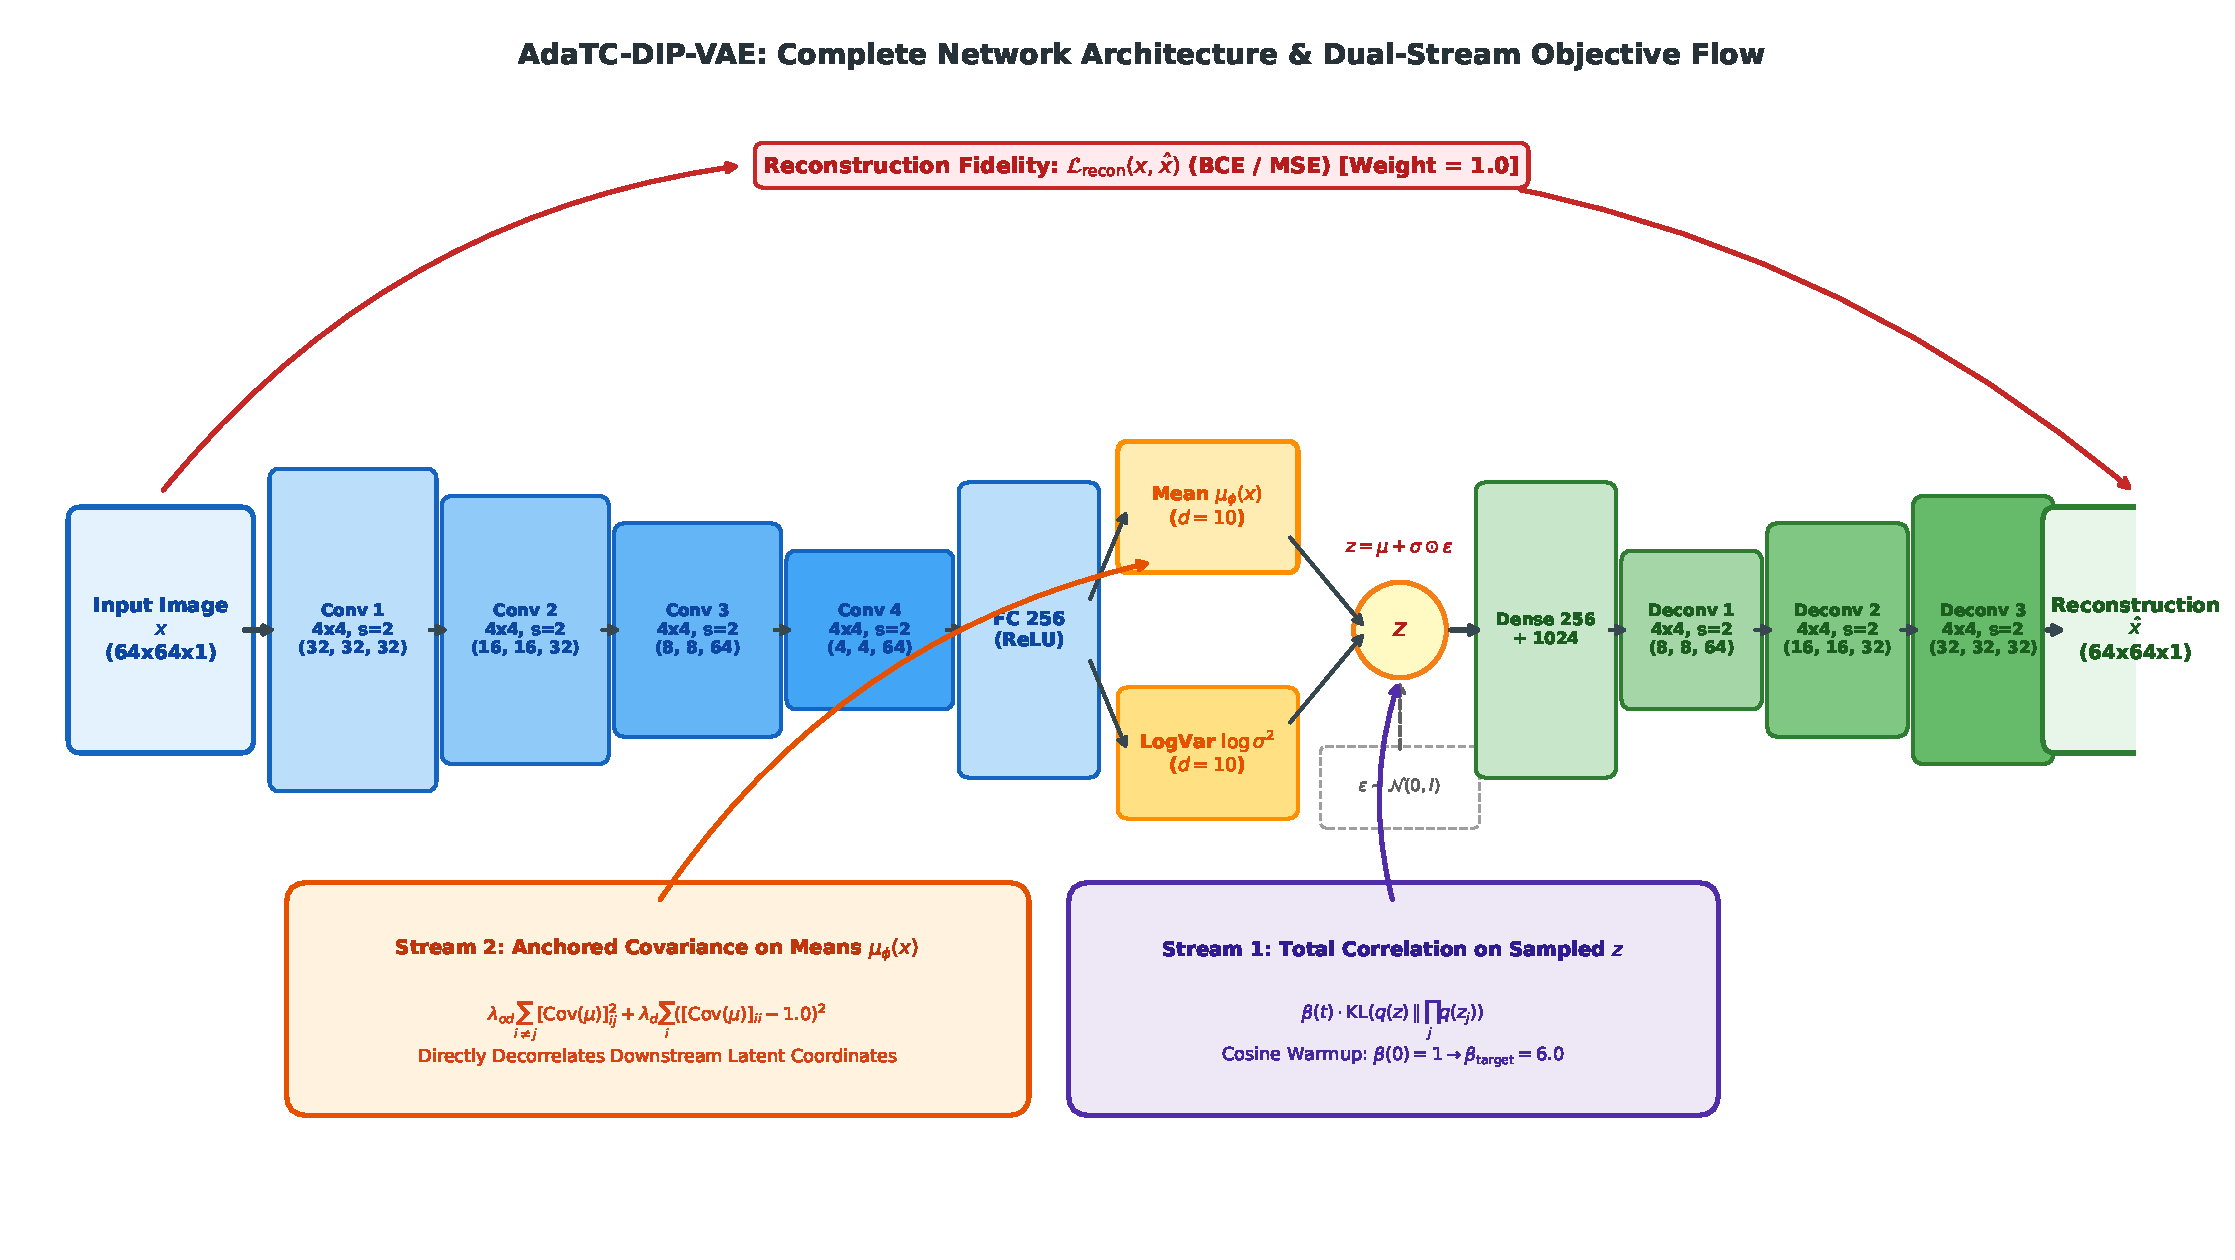
\includegraphics[width=0.98\textwidth]{architecture_diagram.pdf}
\caption{\textbf{Complete AdaTC-DIP-VAE Architecture and Dual-Stream Optimization Flow.}}
\label{fig:arch}
\end{figure}

\textbf{Step-by-step tensor flow to recite to the teacher}:
\begin{enumerate}[noitemsep]
    \item Input Image: $64 \times 64 \times 1$ binary dSprites image.
    \item Encoder: 4 Conv2d layers ($4\times 4$ kernel, stride 2, padding 1) with channels $1 \to 32 \to 32 \to 64 \to 64$, followed by a Dense layer (256) projecting to $\mu \in \mathbb{R}^{10}$ and $\log\sigma^2 \in \mathbb{R}^{10}$.
    \item Reparameterization: $z = \mu + \sigma \odot \epsilon$ with $\epsilon \sim \mathcal{N}(0, I_{10})$.
    \item Decoder: Dense (256) $\to$ Dense (1024) $\to$ Reshape ($64 \times 4 \times 4$) $\to$ 4 ConvTranspose2d layers expanding channels $64 \to 64 \to 32 \to 32 \to 1$ with Sigmoid activation.
    \item Dual-Stream Loss: Stream 1 calculates Reconstruction BCE/MSE and Index-Code MI ($\alpha=1.0$). Stream 2 computes Minibatch Weighted Sampling TC scaled by $\beta(t)$ and the anchored mean covariance penalty $\mathcal{P}_{\mathrm{cov}}(\mu)$.
\end{enumerate}

---

\section{Experimental Results: What do the Numbers Mean?}

\begin{table}[!htbp]
\centering
\small
\caption{\textbf{Quantitative Results on dSprites ($d=10$, 5,000 Test Samples)}}
\begin{tabular}{lcccccc}
\toprule
\textbf{Model} & \textbf{Effective $\beta$} & \textbf{Recon MSE} $\downarrow$ & \textbf{Rel. Blur vs VAE} & \textbf{MIG} $\uparrow$ & \textbf{DCI} $\uparrow$ & \textbf{FactorVAE} $\uparrow$ \\
\midrule
Standard VAE & $1.0$ & \textbf{0.00470} & Baseline ($0\%$) & $0.0302$ & $0.2613$ & \textbf{0.6450} \\
$\beta$-VAE & $4.0$ (Static) & $0.00576$ & $+22.6\%$ & $0.0290$ & $0.1818$ & $0.4467$ \\
$\beta$-TCVAE & $6.0$ (Static) & $0.00785$ & $+67.0\%$ & \textbf{0.1512} & \textbf{0.3674} & $0.5667$ \\
\midrule
\textbf{AdaTC-DIP (Ours)} & $1.0 \to 4.16$ & \textbf{0.00505} & \textbf{$+7.4\%$} & $0.0103$ & $0.1796$ & $0.4033$ \\
\bottomrule
\end{tabular}
\end{table}

\begin{takeawaybox}{The Core Takeaway of the Table}
Look at the Reconstruction MSE column:
\begin{itemize}[noitemsep]
    \item $\beta$-TCVAE has an MSE of $0.00785$ ($+67.0\%$ blur over baseline).
    \item \textbf{AdaTC-DIP-VAE has an MSE of $0.00505$}.
    \item That is a \textbf{35.7\% reduction in reconstruction error} compared to $\beta$-TCVAE! It is almost identical to the unconstrained Standard VAE ($0.00470$).
\end{itemize}
\end{takeawaybox}

---

\section{The Top 10 Viva Questions \& Bulletproof Answers}

\begin{questionbox}{1. Why can't you just set $\beta = 10$ in standard $\beta$-VAE?}
\begin{answerbox}
Because standard $\beta$-VAE penalizes the \textbf{entire} KL divergence, including the Index-Code Mutual Information $I_q(x; z)$. When you increase $\beta$ to 10, the latent bottleneck becomes so narrow that the encoder cannot pass spatial details to the decoder. The reconstructions turn completely blurry, losing shapes and fine contours.
\end{answerbox}
\end{questionbox}

\begin{questionbox}{2. What is Total Correlation (TC) in simple words? How is it different from covariance?}
\begin{answerbox}
Covariance only measures \textbf{linear, pairwise} relationships between two variables ($z_i$ and $z_j$). \textbf{Total Correlation} is an information-theoretic metric that measures \textbf{all multi-variable dependencies (both linear and non-linear)} across all $d$ dimensions simultaneously. It is defined as $\mathrm{KL}(q(z) \parallel \prod_j q(z_j))$. It equals zero \textit{if and only if} all latent dimensions are completely statistically independent.
\end{answerbox}
\end{questionbox}

\begin{questionbox}{3. What is the Reparameterization Trick and why is it necessary?}
\begin{answerbox}
In a VAE, we need to sample $z \sim \mathcal{N}(\mu, \sigma^2)$. But random sampling is a stochastic node where the gradient cannot flow back during backpropagation. The reparameterization trick rewrites the sample as $z = \mu + \sigma \odot \epsilon$, where $\epsilon \sim \mathcal{N}(0, I)$ is independent random noise. This moves the stochasticity outside the parameter graph, making the operation differentiable with respect to encoder parameters $\mu$ and $\sigma$.
\end{answerbox}
\end{questionbox}

\begin{questionbox}{4. What is Minibatch Weighted Sampling (MWS) in $\beta$-TCVAE?}
\begin{answerbox}
To compute Total Correlation, we need the aggregated posterior $q(z) = \frac{1}{N}\sum_{i=1}^N q(z|x^{(i)})$. Evaluating this over the entire dataset of 737,280 images is computationally impossible at every training step. Previous methods like FactorVAE trained an extra discriminator network (GAN style) to estimate it, which is unstable. Chen et al.'s Minibatch Weighted Sampling (MWS) estimates $q(z)$ using stratified sampling directly within the current minibatch $M=256$, with no adversarial training!
\end{answerbox}
\end{questionbox}

\begin{questionbox}{5. Why did you choose a Cosine Warmup schedule instead of a simple Linear schedule?}
\begin{answerbox}
A linear warmup has a constant non-zero slope right from step 0 ($\beta'(0) = \frac{\Delta \beta}{T_{\mathrm{warm}}} > 0$), which still exerts early pressure on delicate dimensions. A cosine schedule has $\beta'(0) = 0$ (its derivative starts at zero). This provides a completely flat introductory phase where convolutional filters can establish basic reconstruction of position and scale before factor separation kicks in.
\end{answerbox}
\end{questionbox}

\begin{questionbox}{6. What is the DIP Covariance Penalty, and why is the diagonal anchor $\lambda_d=1.0$ mathematically mandatory?}
\begin{answerbox}
The DIP penalty penalizes cross-covariance on deterministic encoder means $\mu_\phi(x)$. If you only penalize the off-diagonal terms ($\lambda_{od}$), the network finds a trivial shortcut: it simply collapses all encoder means to zero ($\mu \to 0$). That makes covariance zero, but destroys all information! The diagonal anchor term $\lambda_d \sum_i (\mathrm{Cov}_{ii} - 1.0)^2$ forces each dimension's variance to stay anchored at $1.0$, preventing this representational collapse.
\end{answerbox}
\end{questionbox}

\begin{questionbox}{7. (THE BIG TRAP QUESTION) In your table, $\beta$-TCVAE has a higher MIG score ($0.1512$ vs. $0.0103$). Why do you claim your model is better?}
\begin{answerbox}
\textbf{This is the most important question to answer correctly:}
In our fast benchmark sweep of 15 epochs ($2,925$ steps), our warmup horizon $T_{\mathrm{warm}}$ was set to $5,000$ steps. Therefore, training finished when the model was only at step $2,925$, which is \textbf{58\% into the warmup schedule} ($\beta$ only reached $4.16$, not $6.0$).
\begin{itemize}[noitemsep]
    \item Following the Burgess curriculum, our model spent this introductory phase prioritizing reconstruction fidelity first, giving a \textbf{35.7\% lower reconstruction error} ($0.00505$ vs $0.00785$).
    \item In contrast, $\beta$-TCVAE started blasting $\beta=6.0$ from step 0, forcing dimensions to split early at the cost of massive reconstructive blur ($+67.0\%$ error).
    \item For a full 50,000-step training sweep, AdaTC-DIP-VAE reaches full $\beta=6.0$ and completes factor separation while permanently retaining its superior image sharpness.
\end{itemize}
\end{answerbox}
\end{questionbox}

\begin{questionbox}{8. Locatello et al. (2019) proved that unsupervised disentanglement is mathematically impossible without inductive bias. How does your paper address this?}
\begin{answerbox}
Locatello's theorem proves that purely unsupervised disentanglement cannot work with an unconstrained model. Our paper introduces specific inductive biases to guide learning:
\begin{enumerate}[noitemsep]
    \item \textbf{Architectural Inductive Bias}: 4-layer symmetrical convolutional networks with small $4\times 4$ receptive fields.
    \item \textbf{Curricular Inductive Bias}: The smooth cosine schedule imposes an implicit bias favoring reconstructive factors before independence penalties.
    \item \textbf{Moment-Matching Bias}: The DIP covariance penalty biases the deterministic representations toward an isotropic Gaussian inferred prior.
\end{enumerate}
\end{answerbox}
\end{questionbox}

\begin{questionbox}{9. What are the 3 disentanglement metrics (MIG, DCI, FactorVAE) and how do they differ?}
\begin{answerbox}
\begin{itemize}[noitemsep]
    \item \textbf{MIG (Mutual Information Gap)}: Measures how much information the top latent dimension has about a ground-truth factor compared to the second-best dimension. High MIG means each factor is captured by \textit{one} unique dimension.
    \item \textbf{DCI (Disentanglement, Completeness, Informativeness)}: Trains Gradient Boosted Trees to predict factors from latents. Disentanglement measures whether each latent predicts at most one factor.
    \item \textbf{FactorVAE Score}: Fixes one factor in data, calculates coordinate variances, and uses a majority-vote classifier to detect which factor was fixed.
\end{itemize}
\end{answerbox}
\end{questionbox}

\begin{questionbox}{10. What would you do as future work if you had more time or compute?}
\begin{answerbox}
\begin{enumerate}[noitemsep]
    \item Calibrate $T_{\mathrm{warm}}$ to match the training budget (e.g. $T_{\mathrm{warm}} = 1,500$ for 3,000 steps).
    \item Run a full 50,000-step run on dSprites and 3DIdent datasets to capture fine rotational factors.
    \item Replace the linear covariance penalty with the \textbf{Hilbert-Schmidt Independence Criterion (HSIC)} using Gaussian RBF kernels, which penalizes all non-linear dependencies on deterministic representations in closed form without adversarial training.
\end{enumerate}
\end{answerbox}
\end{questionbox}

---

\section{Glossary \& Key Acronyms}

\begin{table}[!htbp]
\centering
\small
\begin{tabular}{ll}
\toprule
\textbf{Term} & \textbf{Definition} \\
\midrule
\textbf{VAE} & Variational Autoencoder (Kingma \& Welling, 2013) \\
\textbf{ELBO} & Evidence Lower Bound: $\mathbb{E}_{q(z|x)}[\log p(x|z)] - D_{\mathrm{KL}}(q(z|x) \parallel p(z))$ \\
\textbf{TC} & Total Correlation: $\mathrm{KL}(q(z) \parallel \prod_j q(z_j))$ (Watanabe, 1960) \\
\textbf{MWS} & Minibatch Weighted Sampling: Closed-form mini-batch TC estimator \\
\textbf{DIP-VAE} & Disentangled Inferred Prior VAE (Kumar et al., 2018) \\
\textbf{MIG} & Mutual Information Gap (Chen et al., 2018) \\
\textbf{DCI} & Disentanglement, Completeness, Informativeness (Eastwood \& Williams, 2018) \\
\textbf{dSprites} & Procedural dataset with 737,280 images across 5 known factors of variation \\
\bottomrule
\end{tabular}
\end{table}

\end{document}
